The following descriptions preserve the separate secondary populations reported in the main paper. They are not pooled with the fixed-budget comparisons.
Figure~\ref{fig:rq3-outcomes} displays all 108 fixed-budget outcomes. Figure~\ref{fig:rq3-direct-full-absolute} gives absolute costs for every completed Lazy/Direct-Full pair; main-paper Figure~\ref{fig:rq3-paired-absolute} compares Lazy with Eager under the same UC pruning.
% Generated from the fixed rq3-cells.csv and checked against its outcome macros.
\begin{figure}[!htbp]
\centering
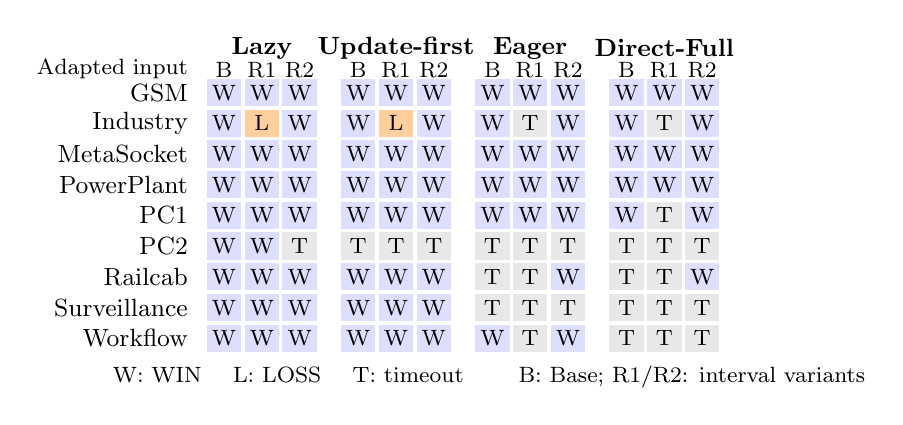
\begin{tikzpicture}[x=.48cm,y=.39cm,font=\small,
    cell/.style={draw=white,minimum width=4.5mm,minimum height=3.6mm,inner sep=0pt,font=\footnotesize},
    win/.style={cell,fill=blue!13,text=black},
    loss/.style={cell,fill=orange!38,text=black},
    timeout/.style={cell,fill=black!9,text=black}]
\node[anchor=east,font=\footnotesize] at (-.7,.75) {Adapted input};
\node[font=\small\bfseries] at (1.00,1.45) {Lazy};
\node[font=\footnotesize] at (0.00,.75) {B};
\node[font=\footnotesize] at (1.00,.75) {R1};
\node[font=\footnotesize] at (2.00,.75) {R2};
\node[win] at (0.00,0.00) {W};
\node[win] at (1.00,0.00) {W};
\node[win] at (2.00,0.00) {W};
\node[win] at (0.00,-1.00) {W};
\node[loss] at (1.00,-1.00) {L};
\node[win] at (2.00,-1.00) {W};
\node[win] at (0.00,-2.00) {W};
\node[win] at (1.00,-2.00) {W};
\node[win] at (2.00,-2.00) {W};
\node[win] at (0.00,-3.00) {W};
\node[win] at (1.00,-3.00) {W};
\node[win] at (2.00,-3.00) {W};
\node[win] at (0.00,-4.00) {W};
\node[win] at (1.00,-4.00) {W};
\node[win] at (2.00,-4.00) {W};
\node[win] at (0.00,-5.00) {W};
\node[win] at (1.00,-5.00) {W};
\node[timeout] at (2.00,-5.00) {T};
\node[win] at (0.00,-6.00) {W};
\node[win] at (1.00,-6.00) {W};
\node[win] at (2.00,-6.00) {W};
\node[win] at (0.00,-7.00) {W};
\node[win] at (1.00,-7.00) {W};
\node[win] at (2.00,-7.00) {W};
\node[win] at (0.00,-8.00) {W};
\node[win] at (1.00,-8.00) {W};
\node[win] at (2.00,-8.00) {W};
\node[font=\small\bfseries] at (4.55,1.45) {Update-first};
\node[font=\footnotesize] at (3.55,.75) {B};
\node[font=\footnotesize] at (4.55,.75) {R1};
\node[font=\footnotesize] at (5.55,.75) {R2};
\node[win] at (3.55,0.00) {W};
\node[win] at (4.55,0.00) {W};
\node[win] at (5.55,0.00) {W};
\node[win] at (3.55,-1.00) {W};
\node[loss] at (4.55,-1.00) {L};
\node[win] at (5.55,-1.00) {W};
\node[win] at (3.55,-2.00) {W};
\node[win] at (4.55,-2.00) {W};
\node[win] at (5.55,-2.00) {W};
\node[win] at (3.55,-3.00) {W};
\node[win] at (4.55,-3.00) {W};
\node[win] at (5.55,-3.00) {W};
\node[win] at (3.55,-4.00) {W};
\node[win] at (4.55,-4.00) {W};
\node[win] at (5.55,-4.00) {W};
\node[timeout] at (3.55,-5.00) {T};
\node[timeout] at (4.55,-5.00) {T};
\node[timeout] at (5.55,-5.00) {T};
\node[win] at (3.55,-6.00) {W};
\node[win] at (4.55,-6.00) {W};
\node[win] at (5.55,-6.00) {W};
\node[win] at (3.55,-7.00) {W};
\node[win] at (4.55,-7.00) {W};
\node[win] at (5.55,-7.00) {W};
\node[win] at (3.55,-8.00) {W};
\node[win] at (4.55,-8.00) {W};
\node[win] at (5.55,-8.00) {W};
\node[font=\small\bfseries] at (8.10,1.45) {Eager};
\node[font=\footnotesize] at (7.10,.75) {B};
\node[font=\footnotesize] at (8.10,.75) {R1};
\node[font=\footnotesize] at (9.10,.75) {R2};
\node[win] at (7.10,0.00) {W};
\node[win] at (8.10,0.00) {W};
\node[win] at (9.10,0.00) {W};
\node[win] at (7.10,-1.00) {W};
\node[timeout] at (8.10,-1.00) {T};
\node[win] at (9.10,-1.00) {W};
\node[win] at (7.10,-2.00) {W};
\node[win] at (8.10,-2.00) {W};
\node[win] at (9.10,-2.00) {W};
\node[win] at (7.10,-3.00) {W};
\node[win] at (8.10,-3.00) {W};
\node[win] at (9.10,-3.00) {W};
\node[win] at (7.10,-4.00) {W};
\node[win] at (8.10,-4.00) {W};
\node[win] at (9.10,-4.00) {W};
\node[timeout] at (7.10,-5.00) {T};
\node[timeout] at (8.10,-5.00) {T};
\node[timeout] at (9.10,-5.00) {T};
\node[timeout] at (7.10,-6.00) {T};
\node[timeout] at (8.10,-6.00) {T};
\node[win] at (9.10,-6.00) {W};
\node[timeout] at (7.10,-7.00) {T};
\node[timeout] at (8.10,-7.00) {T};
\node[timeout] at (9.10,-7.00) {T};
\node[win] at (7.10,-8.00) {W};
\node[timeout] at (8.10,-8.00) {T};
\node[win] at (9.10,-8.00) {W};
\node[font=\small\bfseries] at (11.65,1.45) {Direct-Full};
\node[font=\footnotesize] at (10.65,.75) {B};
\node[font=\footnotesize] at (11.65,.75) {R1};
\node[font=\footnotesize] at (12.65,.75) {R2};
\node[win] at (10.65,0.00) {W};
\node[win] at (11.65,0.00) {W};
\node[win] at (12.65,0.00) {W};
\node[win] at (10.65,-1.00) {W};
\node[timeout] at (11.65,-1.00) {T};
\node[win] at (12.65,-1.00) {W};
\node[win] at (10.65,-2.00) {W};
\node[win] at (11.65,-2.00) {W};
\node[win] at (12.65,-2.00) {W};
\node[win] at (10.65,-3.00) {W};
\node[win] at (11.65,-3.00) {W};
\node[win] at (12.65,-3.00) {W};
\node[win] at (10.65,-4.00) {W};
\node[timeout] at (11.65,-4.00) {T};
\node[win] at (12.65,-4.00) {W};
\node[timeout] at (10.65,-5.00) {T};
\node[timeout] at (11.65,-5.00) {T};
\node[timeout] at (12.65,-5.00) {T};
\node[timeout] at (10.65,-6.00) {T};
\node[timeout] at (11.65,-6.00) {T};
\node[win] at (12.65,-6.00) {W};
\node[timeout] at (10.65,-7.00) {T};
\node[timeout] at (11.65,-7.00) {T};
\node[timeout] at (12.65,-7.00) {T};
\node[timeout] at (10.65,-8.00) {T};
\node[timeout] at (11.65,-8.00) {T};
\node[timeout] at (12.65,-8.00) {T};
\node[anchor=east] at (-.7,0.00) {GSM};
\node[anchor=east] at (-.7,-1.00) {Industry};
\node[anchor=east] at (-.7,-2.00) {MetaSocket};
\node[anchor=east] at (-.7,-3.00) {PowerPlant};
\node[anchor=east] at (-.7,-4.00) {PC1};
\node[anchor=east] at (-.7,-5.00) {PC2};
\node[anchor=east] at (-.7,-6.00) {Railcab};
\node[anchor=east] at (-.7,-7.00) {Surveillance};
\node[anchor=east] at (-.7,-8.00) {Workflow};
\node[anchor=west,font=\footnotesize] at (-3.2,-9.25)
  {W: WIN \quad L: LOSS \quad T: timeout \qquad B: Base; R1/R2: interval variants};
\end{tikzpicture}
\caption{Every fixed-budget contract--method outcome. Each tile is one of the same
\ApplicationModels{} inputs $\times$ three requirement variants, under a
1,200~s cap and 64~GiB heap. WIN and LOSS are completed decisions; timeout leaves
feasibility unresolved. The methods change exploration, keeping entries,
successors and goals fixed. The comparison evaluates complete exploration procedures.
Workflow/R2's Direct-Full tile uses the recorded same-setting timeout after
interruption; both attempts are retained.}
\label{fig:rq3-outcomes}
\Description{A grid of all 27 contracts for each of four methods. Lazy has 25 WIN,
one LOSS at Industry R1 and one timeout at PC2 R2. Update-first has 23 WIN, one LOSS
and three timeouts. Eager has 17 WIN and ten timeouts. Direct-Full has 14 WIN and
13 timeouts. Every completed paired decision agrees.}
\end{figure}

\FloatBarrier
Base/R1/R2's 5/3/6 pairs give median state ratios 111.89/11.88/2.75 and solver ratios 40.02/3.12/9.14. The largest state savings are in Base, but different completed populations do not isolate interval requirements' effect.

\paragraph{Order sensitivity in R2.}
Eight R2 contracts complete all five repetitions with both Lazy and Update-first; PC2/R2 times out with both. Update-first discovers fewer states and has a lower solver median on Industry, PowerPlant, PC1, Railcab, Surveillance and Workflow; Lazy is lower on both measures for GSM and MetaSocket. For example, PC1/R2 has 56,443 versus 9,304 discovered states and 6.155 versus 1.166 seconds for Lazy versus Update-first. These saved results expose a substantial order dependence, but do not isolate a causal interaction between the order and interval monitors. The performance contribution concerns the full lazy procedure relative to construction alternatives, not a uniformly best exploration order.

\subsection{Complete records for the separate populations}
Supplement Sections~\ref{suppDoc-supp:vthree-ablations} and~\ref{suppDoc-supp:scaling} retain all Full+UC, restricted-transfer, controlled-family and Travel outcomes. Full+UC mixes builds, hosts and repetitions; its timing does not isolate UC pruning. For Legacy's subsequent-control reference, fixed-budget OOM/unmeasured cells are in Supplement Section~\ref{suppDoc-supp:fixed-budget}, source/fork discrepancies in Section~\ref{suppDoc-supp:legacy-reference}, and separate enlarged-heap trials in Section~\ref{suppDoc-supp:vthree-ext-six}. Other enlarged-budget failures and skips are in Appendix~\ref{ta:extended_budget} and Supplement Section~\ref{suppDoc-supp:extended-budget}; none enters fixed-budget medians.

The boundary fixture distinguishes forbidding an intervening event from merely merging same-type boundary labels (Supplement Section~\ref{suppDoc-supp:boundary-inputs}); Cell$_n$ and restricted-transfer controls follow in Section~\ref{suppDoc-supp:vthree-ablations}. The original finite-file results remain in Section~\ref{suppDoc-supp:independent-checks}; Section~\ref{suppDoc-supp:vthree-ablations} retains earlier failed inputs. Supplement Sections~\ref{suppDoc-supp:industry-diagnostic} and~\ref{suppDoc-supp:railcab-exports} give the complete Industry losing-region and Railcab policy diagnoses. Industry's global losing closure excludes every order; the validation-permitting variant changes the contract and supplies no timing data. The native DUCS WIN uses a different subsequent-control objective (main-paper Section~\ref{sec:railcab-policy}).

\subsection{Input adaptation details}
Nine inputs manually adapt eight DUCS sources; both ProductionCell sizes share a parent. Base/R1/R2 vary interval requirements, fixing components, transfers, endpoints and old/new goals (Technical Appendix~\ref{ta:benchmark_inputs}). Adaptations make PC tool results UC, revise Surveillance battery behavior/safety, order GSM/R2's decode boundaries before ENV transfer, shorten Railcab transfer paths while keeping both outcomes, and omit PowerPlant's explicit \texttt{ENV\_OLD}-to-\texttt{ENV\_NEW} transfer declaration while retaining \texttt{STARTED}-to-\texttt{STARTED}; the environment names alias those initial states. Recorded provenance does not establish whole-problem equivalence.

PC1/PC2 retain their DUCS parent's repeatable arrival cycle: UC $in_i$ enters an occupied arm; controllable $out_i$ and UC $reset_i$ permit its next arrival. With work and output withheld, pending tool results or reset/arrival chains finish in quiescent arm states. PC2-Rolling adds one UC calibration-completion step. This is finite drainage of pending physical events, not a total arrival budget or a safety proof. DUCS's production-cell study likewise distinguishes an empty-line condition from delaying newly arrived raw work~\cite[Sec.~6.1]{Nahabedian2020}. FG commands require no enabled UC event; a temporal gap between arrivals alone does not ensure this.

Travel couples an agency with $N$ amenities, $K$ UC choices and $0$--$K-1$ selection steps: size, branching and length covary. Adaptations change purchasing, admission, transfers and monitors without claimed trace equivalence. Supplement Section~\ref{suppDoc-supp:scaling} retains every setting and completed-pair comparison; $(N,K)=\FixedTravelAdditionalSettingsMath{}$ are the only settings extending OTF's fixed-budget decided range.

\paragraph{Independent-update construction.}
The complete $n+1$ versus $2^n$ construction and its proof occur once, in Supplement Section~\ref{suppDoc-supp:independent-family}. It assumes the measured pending-transfer-first query order and supplies no order-independent performance guarantee.

\subsection{Memory and returned policies}\label{ta:memory_policies}
Lazy's five-run median peak working sets span \FixedLazyRSSMin{}--\FixedLazyRSSMax{}~GiB (median \FixedLazyRSSMedian{}), including JVM/native overhead; Eager/Update-first sometimes use less. Its \FixedPolicies{} WIN certificates contain \FixedPolicyStatesMin{}--\FixedPolicyStatesMax{} update states (median \FixedPolicyStatesMedian{}) and maximum ranks \FixedRankMin{}--\FixedRankMax{} (median \FixedRankMedian{}). Ranks bound events, not downtime or optimal length. Counts match all five repeats; LOSS/TO has no winning policy.

The rank domain is recorded as \texttt{certificate\_states} in saved \path{rq3/stage1.csv}. S4's ``Output policy states'' instead uses \texttt{output\_controller\_states}: the linked old--update--new controller, with 15--1,260 states for Lazy. Linking includes reachable old and new closed-loop states and non-goal update states, identifying each update goal with its selected new state. These columns describe the same successful runs at different construction stages; neither counts explored game states.

\subsection{Lifetime gaps in two saved policies}\label{ta:saved-gaps}
The separate qualitative Railcab Base/R1 exports in S4 retain their full policy graphs. Define a gap on a completed path as the labels strictly after its last old-stop edge and strictly before its first new-start edge, excluding both boundaries. A normal label is outside the complete command set pending at entry. All 22 entries of each export have every old stop before the first new start on every possible policy path. There are 34 Base and 41 R1 completed paths when paths from different old entries are counted separately.
\begin{center}\small
\begin{tabular}{@{}lrrrr@{}}\toprule
Saved policy & States / edges & Entries & Gap labels & Ordinary gap labels\\\midrule
Railcab Base & 115 / 118 & 22 & 5--8 & 1--4\\
Railcab R1 & 44 / 46 & 22 & 3 & 0\\\bottomrule
\end{tabular}
\end{center}
The Base policy exploits a period without old or new requirements; R1 keeps its seven interval monitors active even when those requirements are inactive. The observed zero ordinary events in R1 describes this selected policy, not every winning policy. These counts quantify events, not elapsed time or suppressed alternatives.

The revised source's \path{scripts/analyze_saved_railcab_gap.py} traverses every saved outcome from every entry. It verifies entry coverage, strict rank decrease, one-shot command consumption, active-monitor membership, full certificate reachability and all terminal paths. Its inputs are the two \path{handoff-bundle.json} files under \path{results/supplement-checks/railcab_policy_demo/} and \path{results/supplement-checks/railcab_r1_policy_demo/}; it returns per-entry ranges and extremal path segments. Counting internal edges of the region with no active old/new monitor independently gives the same ranges for all 44 entries. The input bundles and this analysis script are included in the matching public snapshot.

This is a static analysis of the already saved qualitative exports, with no new synthesis or timing trial. Lazy's 125 successful fixed-budget repetitions instead retain summary-only controller output, certificate sizes and maximum ranks. Their unrecorded policy edges cannot establish corresponding gap ranges for all 25 WIN contracts. Neither these two exports nor their analysis reconstructs enabled but unselected events or an optimal completion rank.
